\documentclass[12pt]{article}
\usepackage[margin=2.5cm]{geometry}
\usepackage{enumerate}
\usepackage{amsfonts}
\usepackage{amsmath}
\usepackage{fancyhdr}
\usepackage{amsmath}
\usepackage{amssymb}
\usepackage{amsthm}
\usepackage{mdframed}
\usepackage{graphicx}

\begin{document}
\title{Worksheet 19 Solution}
\author{Hyungmo Gu}
\maketitle

\section*{Question 1}
\begin{enumerate}[a.]
    \item
    By the figure below, we can conclude there are 7 vertices.

    \begin{center}
    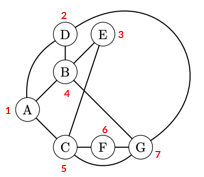
\includegraphics[width=6cm]{images/worksheet_19_q1a_solution.png}
    \end{center}

    \item
    By the figure below, we can conclude there are 11 edges.

    \begin{center}
    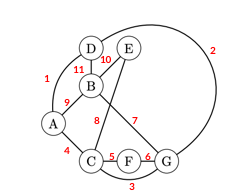
\includegraphics[width=6cm]{images/worksheet_19_q1b_solution.png}
    \end{center}

    \newpage
    \item
    By the figure below, we can conclude there are 4 vertices adjacent to G.

    \begin{center}
    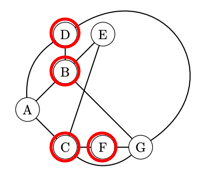
\includegraphics[width=6cm]{images/worksheet_19_q1c_solution.png}
    \end{center}

\end{enumerate}

\section*{Question 2}

\section*{Question 3}

\end{document}